\section{Auswertung}
\label{sec:Auswertung}

\subsection{Statische Methode}

In \autoref{fig:45grad1} ist zu erkennen, dass beide Temperaturen ähnlich verlaufen, doch ist die Temperatur am Abtastpunkt T4 durchschnittlich 11.908\% kleiner.

\begin{figure}
    \centering
    \includegraphics[scale=0.7]{build/plot1.pdf}
    \caption{Die Temperaturverläufe von Messing  weisen eine ähnliche logarithmische Steigung auf. Dabei steigt T4 langsamer an als T1.}
    \label{fig:45grad1}
\end{figure}

%\newpage
Sehr ähnlich verlaufen auch die Temperaturen in \autoref{fig:45grad2}, wobei hier T5 deutlich stärker ansteigt als T8.
Die Temperaturkurven haben einen durchschnittlichen Unterschied von 27.499\% voneinander.

\begin{figure}
    \centering
    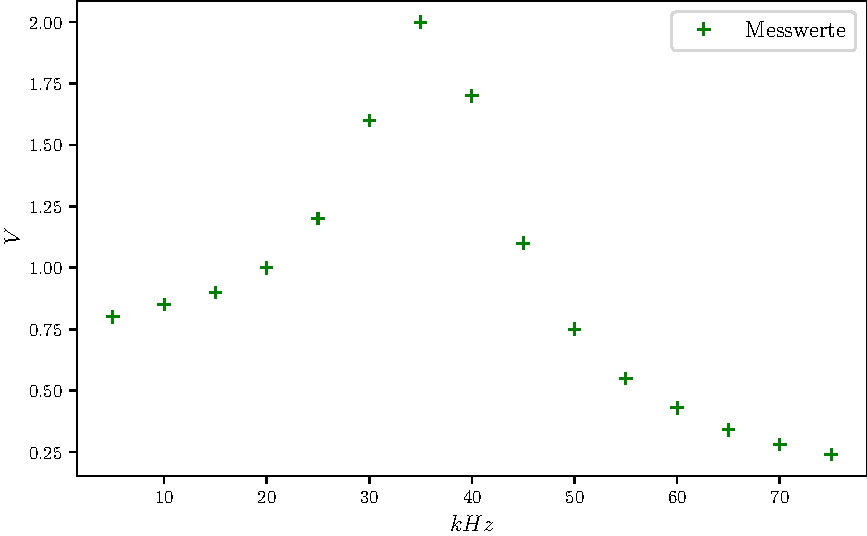
\includegraphics[scale=0.7]{build/plot2.pdf}
    \caption{Die Temperaturverläufe von Aluminium und Edelstahl steigen ebenfalls logarithmisch an, wobei Edelstahl deutlich langsamer an Hitze gewinnt.}
    \label{fig:45grad2}
\end{figure}

%\newpage
Die Temperatur der Thermoelemente am Ende der Messung bei $425\ s$ betragen:

\begin{itemize}
    \centering
    \item[] $T1 = 48.74\ °C$ 
    \item[] $T4 = 50.14\ °C$
    \item[] $T5 = 50.37\ °C$
    \item[] $T8 = 35.64\ °C$
\end{itemize}

Die beste Wärmeleitung hat demnach Aluminium am Abgriff T5.\\
Um den Wärmestrom $\Delta Q/\Delta t$ zu berechnen, braucht es die Werte der Wärmeleitfähigkeit für die verschiedenen Materialien \cite{web}, sowie den Querschnitt der Metalle und den Abstand der Abgriffstellen.
\newpage
\begin{itemize}
    \centering
    \item[] $\kappa_{Messing} = 111\ \frac{W}{m\cdot K}$
    \item[] $A_{Messing(breit)} = 48\cdot 10^{-6}\ m^2$
    \item[] $\Delta x_{Messing(breit)} = 0.03\ m$ 
    \item[] 
    \item[] $\kappa_{Edelstahl} = 14.4\ \frac{W}{m\cdot K}$
    \item[] $A_{Edelstahl} = 48\cdot 10^{-6}\ m^2$
    \item[] $\Delta x_{Edelstahl} = 0.03\ m$
    \item[] 
    \item[] $\kappa_{Aluminium} = 237\ \frac{W}{m\cdot K}$
    \item[] $A_{Aluminium} = 48\cdot 10^{-6}\ m^2$
    \item[] $\Delta x_{Aluminium} = 0.03\ m$
    \label{it:item} 
\end{itemize}

Daraus ergeben sich für 5 zufällige Messzeiten mithilfe der \autoref{eq:warmcurrent} folgende Wärmeströme in \autoref{tab:warmcurrent}.

\begin{table}
    \centering
    \caption{Tabelle des Wärmestroms für 5 versch. Messzeiten.}
    \begin{tabular}{c|c|c|c|c}
        \toprule
        Messzeit [s] & $\Delta T = T2\ -\ T1$ [K] & $\frac{\Delta Q}{\Delta t}_{12}\ [W]$ & $\Delta T = T7\ -\ T8$ [K] & $\frac{\Delta Q}{\Delta t}_{78}\ [W]$\\
        \midrule
        50 & 5.73 & -1.02 & 5.17 & -0.119\\
        100 & 5.32 & -0.94 & 9.19 & -0.212\\
        150 & 4.48 & -0.796 & 10.51 & -0.242\\
        200 & 3.87 & -0.687 & 10.69 & -0.246\\
        250 & 3.42 & -0.607 & 10.48 & -0.241\\
    \end{tabular}
    \label{tab:warmcurrent}
\end{table}

\begin{figure}
    \centering
    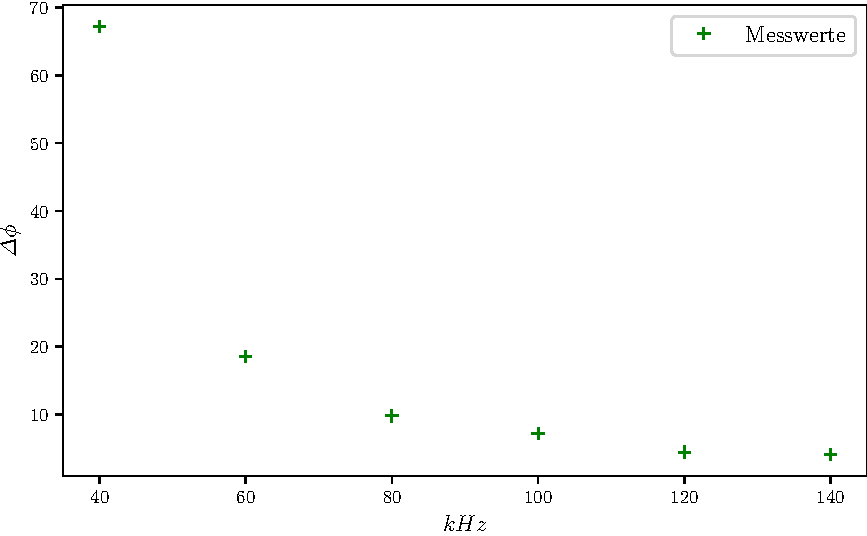
\includegraphics[scale=0.7]{build/plot3.pdf}
    \caption{Plot der Differenzen der Temperatur von Messing und Edelstahl.}
    \label{fig:deltaT}
\end{figure}
In \autoref{fig:deltaT} ist die Differenz der Temperaturen dargestellt, die in \autoref{tab:warmcurrent} zur Berechnung verwendet wurden.

\newpage
\subsection{Dynamische Methode}
Die \autoref{fig:dynamic1} zeigt die Temperaturverläufe von beiden Abgriffstellen des breiten Messingstabs.
Um die notwendigen Amplituden für die Berechnung der Wärmeleitfähigkeit $\kappa$ zu bestimmen, wird jede einzelne Amplitude per Hand vermessen und berechnet.
Die Extrema werden hierbei mithilfe von \textit{Scipy.signal.argrelextrema} bestimmt.

\begin{figure}[htbp]
    \centering
    \includegraphics[scale=1]{build/plot4.pdf}
    \caption{Temperaturverlauf des breiten Messingstabs bei einer Periodendauer von $80\ s$.}
    \label{fig:dynamic1}
\end{figure}

In \autoref{tab:ampl} sind die korrekten Amplituden für beide Abgriffstellen verzeichnet.

\begin{table}[htbp]
    \centering
    \caption{Es sind $A_{nah}$, $A_{fern}$, sowie der ausgerechnete natürliche Logarithmus und die Phasendifferenz aufgelistet.}
    \label{tab:ampl}
    \begin{tabular}{c|c|c|c}
        \toprule
        $A_{nah}\pm 0.1$ [$K$] & $A_{fern}\pm 0.1$ [$K$] & $ln(\frac{A_{nah}}{A_{fern}})$ & Phasendifferenz $\Delta t$ [$s$]\\
        \midrule
        2.25 & 0.5 & $1.504\pm 0.205$ & 25\\
        2.5 & 0.75 & $1.204\pm 0.139$ & 20\\
        2.5 & 0.9 & $1.022\pm 0.118$ & 15\\
        2.55 & 1.0 & $0.936\pm 0.107$ & 15\\
        2.6 & 1.1 & $0.860\pm 0.099$ & 15\\
        2.7 & 1.15 & $0.853\pm 0.095$ & 15\\
        2.75 & 1.15 & $0.872\pm 0.094$ & 15\\
        \bottomrule
    \end{tabular}
\end{table}
\newpage
Die benötigten und gemittelten Daten von \autoref{tab:ampl} für die Berechnung der Wärmeleitfähigkeit $\kappa_{Messing}$ lauten:

\begin{itemize}
    \centering
    \item[] $ln(\frac{A_{nah}}{A_{fern}}) = 1.04\pm 0.05$ 
    \item[] $\Delta t = 17.143\ s\pm 1.487\ s$
    \item[] $\Delta x = 0.03\ m$
    \item[] $\rho = 8520\ \frac{kg}{m^3}$
    \item[] $c = 385\ \frac{J}{kg\cdot K}$
\end{itemize}

Daraus ergibt sich nach \autoref{eq:warleit}:
 
\begin{equation}
    \kappa_{Messing} = 83\pm 8\ \frac{W}{m\cdot K}
\end{equation}

Bei allen Berechnungen wurden die Unsicherheiten mit \autoref{eq:gauß} und \textit{Python 3.7, uncertainties} ausgerechnet.
\newpage
Die \autoref{fig:dynamic2} zeigt die Temperaturverläufe von Aluminium an beiden Abgriffstellen.
Wie zuvor bei Messing werden hier ebenfalls die Amplituden einzeln vermessen und in \autoref{tab:ampl2} zusammen mit Logarithmus und Phasenverschiebung aufgelistet.

\begin{figure}[htbp]
    \centering
    \includegraphics{build/plot5.pdf}
    \caption{Temperaturverlauf von Aluminium bei einer Periodendauer von $80\ s$.}
    \label{fig:dynamic2}
\end{figure}

\begin{table}
    \centering
    \caption{Tabelle der Amplituden und Phasenverschiebung von Aluminium.}
    \label{tab:ampl2}
    \begin{tabular}{c|c|c|c}
        \toprule
        $A_{nah}\pm 0.1$ [$K$] & $A_{fern}\pm 0.1$ [$K$] & $ln(\frac{A_{nah}}{A_{fern}})$ & Phasendifferenz $\Delta t$ [$s$]\\
        \midrule
        1.9 & 0.9 & $0.747\pm 0.123$ & 15\\
        2.35 & 1.25 & $0.631\pm 0.091$ & 10\\
        2.5 & 1.5 & $0.511\pm 0.078$ & 10\\
        2.55 & 1.5 & $0.531\pm 0.077$ & 10\\
        2.5 & 1.6 & $0.446\pm 0.074$ & 5\\
        2.65 & 1.6 & $0.505\pm 0.073$ & 5\\
        2.75 & 1.65 & $0.511\pm 0.071$ & 5\\
        \bottomrule
    \end{tabular}
\end{table}
\newpage
Für die Berechnung der Wärmeleitfähigkeit von Aluminium sind die Werte

\begin{itemize}
    \centering
    \item[] $ln(\frac{A_{nah}}{A_{fern}}) = 0.555\pm 0.032$
    \item[] $\Delta t = 8.571\ s\pm 1.429\ s$
    \item[] $\Delta x = 0.03\ m$
    \item[] $\rho = 2800\ \frac{kg}{m^3}$
    \item[] $c = 830\ \frac{J}{kg\cdot K}$
\end{itemize}

in \autoref{eq:warleit} einzusetzen.\\
Die Wärmeleitfähigkeit für Aluminium ist somit:
 
\begin{equation}
    \kappa_{Aluminium} = 220\pm 40\ \frac{W}{m\cdot K}
\end{equation}

Die Periodendauer der Messung von Edelstahl betrug $200\ s$, bis eines der  acht Abtastpunkte $80\ °C$ erreichte, sodass möglichst viele Zyklen gemessen werden konnten.
In \autoref{fig:dynamic3} ist der Temperaturverlauf von den Abtastpunkten T7 und T8 aufgetragen, sowie die Maxima.

\begin{figure}[htbp]
    \centering
    \includegraphics{build/plot6.pdf}
    \caption{Verlauf der Temperatur von Edelstahl bei einer Periodendauer von $200\ s$.}
    \label{fig:dynamic3}
\end{figure}

Bei der \autoref{tab:ampl3} sind, wie bei Messing und Aluminum, die Amplituden und der Logarithmus, sowie die Phasenverschiebung aufgetragen.

\begin{table}
    \centering
    \caption{Tabelle der Amplituden und Phasenverschiebung von Edelstahl.}
    \label{tab:ampl3}
    \begin{tabular}{c|c|c|c}
        \toprule
        $A_{nah}\pm 0.5$ [$K$] & $A_{fern}\pm 0.25$ [$K$] & $ln(\frac{A_{nah}}{A_{fern}})$ & Phasendifferenz $\Delta t$ [$s$]\\
        \midrule
        4 & 0.5 & $2.079\pm 0.515$ & 115\\
        4.5 & 0.5 & $2.197\pm 0.512$ & 100\\
        5 & 0.75 & $1.897\pm 0.348$ & 90\\
        5 & 0.75 & $1.897\pm 0.348$ & 80\\
        5.5 & 1 & $1.705\pm 0.266$ & 80\\
        5.5 & 1 & $1.705\pm 0.266$ & 75\\
        5.5 & 1.25 & $1.482\pm 0.22$ & 75\\
        5.75 & 1.25 & $1.526\pm 0.218$ & 70\\
        5.75 & 1.25 & $1.526\pm 0.218$ & 65\\
        5.75 & 1.5 & $1.344\pm 0.188$ & 65\\
        5.5 & 1.5 & $1.299\pm 0.19$ & 65\\
        5.75 & 1.5 & $1.344\pm 0.188$ & 65\\
        5.5 & 1.5 & $1.299\pm 0.19$ & 65\\
        5.75 & 1.75 & $1.19\pm 0.167$ & 65\\
        5.75 & 1.75 & $1.19\pm 0.167$ & 70\\
        \bottomrule
    \end{tabular}
\end{table}
\newpage
Damit liegen die benötigten, gemittelten Werte bei:

\begin{itemize}
    \centering
    \item[] $ln(\frac{A_{nah}}{A_{fern}}) = 3.38\pm 0.16$
    \item[] $\Delta t = 76.333\ s\pm 3.857\ s$
    \item[] $\Delta x = 0.03\ m$
    \item[] $\rho = 8000\ \frac{kg}{m^3}$
    \item[] $c = 400\ \frac{J}{kg\cdot K}$
\end{itemize}

Daraus ergibt sich für die Wärmeleitfähigkeit von Edelstahl:

\begin{equation}
    \kappa_{Aluminium} = 5.6\pm 0.4\ \frac{W}{m\cdot K}
\end{equation}